\subsection{Émulation par interception}
\label{section:interception}
%% principe: interception des actions et médiation (pas juste interception et rejeu). Intercepter des symboles pour en changer l'effet

Dans le cas de l'émulation par interception, illustrée
Fig.\ref{TYPE_VIRTUALISATION}, pour mettre en place un environnement distribué
émulé sur lequel les applications penseront s'exécuter, deux outils vont être
utilisés; un simulateur pour virtualiser l'environnement d'exécution, et un
émulateur qui va attraper toutes les communications de l'application avec l'hôte
et qui les transmettra ensuite au simulateur.
%%  Les calculs de l'application seront effectués sur la machine hôte
%% mais c'est le simulateur qui calculera le temps de réponse à l'application. Pour
%% cela il fera un rapport entre le temps d'exécution du calcul sur la machine hôte
%% (fourni par l'émulateur qui le mesure lors de l'exécution du calcul), la
%% puissance de l'hôte et celle des machines de l'environnement que l'on simule. Le
%% temps de l'application sera donc celui du simulateur et non le temps réel. En
%% effet, \textit{si on se base sur l'horologe de la machine hôte pour gérer le
%%   temps de l'application, il faudra pour chaque calcul trouver la différence de
%%   temps entre l'exécution sur l'hôte et celle sur la plateforme émulée pour
%%   décaler l'horloge de l'application et maintenir la virtualisation de
%%   l'environnement distribué. Avec cette solution on ne se contente pas de faire
%%   de l'interception d'action et du rejeu par l'émulateur comme c'est le cas avec
%%   l'émulation par limitation. On va intercepter les actions des applications et
%%   les modifier avant de les laisser s'exécuter sur la plateforme réelle sous le
%%   contrôle de l'émulateur pour maintenir la vision d'un environnement distribuée
%%   pour l'application. Ce mécanisme s'appelle la médiation.}

 Une application distribuée peut vouloir communiquer avec l'hôte soit pour
 effectuer de simples calculs %% {\color{red}\textbf{TODO}}(SEB)
 , soit pour effectuer des requêtes de
 connexion ou de communication avec d'autres applications sur le réseau. Quand
 l'émulateur intercepte une communication venant d'un des processus d'une
 application, il modifie les caractéristiques de cette dernière pour qu'elle
 puisse s'exécuter sur la machine hôte. Quand cette dernière renvoie une réponse
 à l'application, elle est également interceptée par l'émulateur pour que
 l'application ne voit pas le changement d'architecture. En même temps, il
 envoie au simulateur le temps d'exécution de l'action sur la machine hôte pour
 qu'il puisse calculer ce temps sur la machine simulée, en faisant un rapport
 entre les performances des deux machines. Les délais calculés par le simulateur
 sont soit des temps de calculs soit des temps de connexion ou de
 communication. Lorsque le simulateur a terminé le calcul du temps de réponse,
 il le transmet à l'émulateur qui l'envoie à l'application en plus du résultat
 du calcul demandé pour mettre à jour son horloge. Ainsi, les calculs sont
 réellement exécutés sur la machine, les communications réellement émises sur le
 réseau géré par le simulateur et c'est le temps de réponse qu'il fourni qui va
 influencer l'horloge de l'application. Finalement, les applications ne
 communiquent plus directement entre elles.

 \begin{figure}
   \centering
   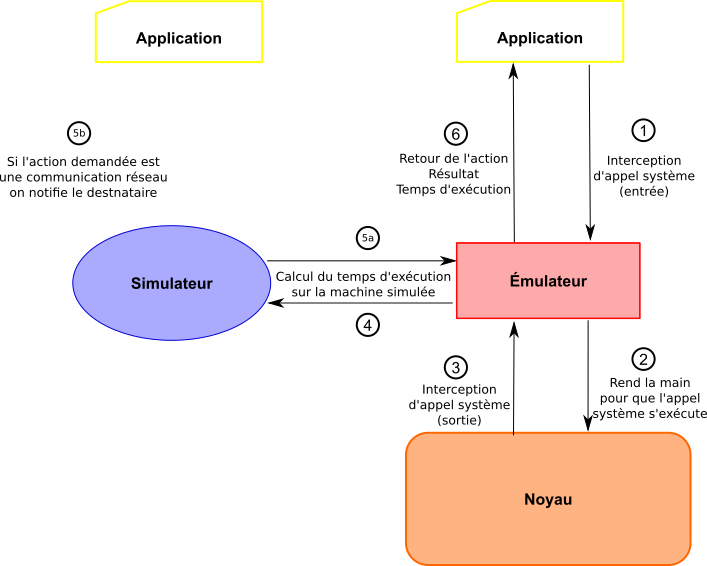
\includegraphics[scale=0.5]{Pictures/png/Emulation_fonctionnement}
   \caption{Fonctionnement de l'émulation par interception}
   \label{INTERCEPTION}
 \end{figure}
 
Pour intercepter ces actions, il faut d'abord choisir à quel niveau se placer.
%% : code source ou binaire. Mais il faut également choisir sur quel
%% type de symbole (appel système, appel de fonction...), utilisé par l'application
%% pour exécuter ses actions, et avec quel outil l'émulateur fera des modifications permettant de maintenir la vision d'un environnement distribué. Par la suite on a ppelera médiation l'ensemble de ces modifications.
%%     qui suit l'interception et avec quel
%% outil.
 En effet, une application peut communiquer avec le noyau via différentes
 abstractions. Elle peut soit utiliser les fonctions d'interaction directe avec
 le noyau que sont les appels systèmes, soit utiliser les différentes
 abstractions fournies par le système d'exploitation: bibliothèques (fonctions
 de la libc par exemple) ou les fonctions POSIX dans le cas d'un système UNIX.

\begin{figure}[H]
 \centering
 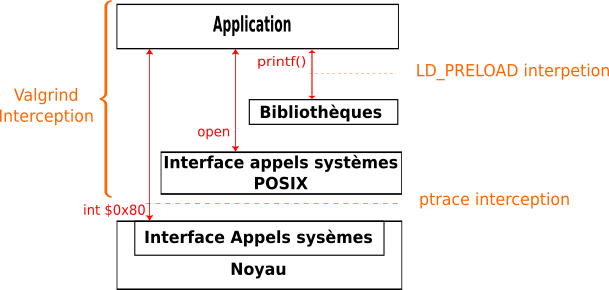
\includegraphics[scale=0.75]{Pictures/png/Communication_application_noyau_v3.png}
 \caption{Communications possibles entre le noyau et une application}
 \label{AS_Communication}
\end{figure}

Nous allons donc voir comment on peut intercepter et modifier des actions au
niveau de l'application (fichier source puis binaire), des appels systèmes et
des appels de fonctions. Par la suite nous appelerons médiation l'ensemble des
modifications effectuées par l'émulateur sur les actions interceptées.
%% {\color{red} L'interception des actions d'une application peut se faire à deux niveaux: sur le fichier source et sur le binaire. La médiation qui suit l'interception des actions peut également se faire sur différent type de symboles: les appels de focntions et les appels systèmes.  \textit{mettre partie ce qu'on intercepte pourquoi et le schéma}}
